\documentclass[17pt,aspectratio=169]{beamer}

\usepackage[T1,T2A]{fontenc}
\usepackage[utf8]{inputenc}
\usepackage[english,russian]{babel}
\usepackage{textcomp}
\usepackage[normalem]{ulem}
\usepackage{hyperref} 

\usetheme{Madrid}

\usepackage{graphicx}

\usepackage{xcolor}
\definecolor{bluekeywords}{rgb}{0,0,1}
\definecolor{greencomments}{rgb}{0,0.5,0}
\definecolor{redstrings}{rgb}{0.64,0.08,0.08}
\definecolor{xmlcomments}{rgb}{0.5,0.5,0.5}
\definecolor{types}{rgb}{0.17,0.57,0.68}

\usepackage{listings}
\lstset{
language=[Sharp]C, 
showspaces=false,
showtabs=false,
breaklines=true,
showstringspaces=false,
breakatwhitespace=true,
escapeinside={(*@}{@*)},
morekeywords={partial, var, value, get, set, async, await, Task},
commentstyle=\color{greencomments},
keywordstyle=\color{bluekeywords},
stringstyle=\color{redstrings},
basicstyle=\ttfamily\small
}

\AtBeginSection[]{
  \begin{frame}
  \vfill
  \centering
  \begin{beamercolorbox}[sep=8pt,center,shadow=true,rounded=true]{title}
    \usebeamerfont{title}\insertsectionhead\par%
  \end{beamercolorbox}
  \vfill
  \end{frame}
}

\title{HttpClient} 
\subtitle{основные ошибки и способы их избежать}
\author{Риваль Абдрахманов}
\institute[PT]{Positive Technologies} 
\date{SpbDotNet, 2019}

\begin{document}
\begin{frame}
\titlepage
\end{frame}

\begin{frame}
\frametitle{Содержание}
\tableofcontents
\end{frame}

\section{HttpClient - базовая информация}

\begin{frame}{\href{https://docs.microsoft.com/en-us/dotnet/api/system.net.http.httpclient?view=netcore-2.2}{HttpClient Class}}
    \begin{itemize}
        \item <1-> Базовый класс для отправки HTTP-запросов и получения HTTP-ответов;
        \item <2-> $GetAsync(\ldots)$, $PostAsync(\ldots)$, $SendAsync(\ldots)$ и др.;
        \item <3-> $HttpClient$ реализует $IDisposable$.
    \end{itemize}
\end{frame}

\begin{frame}{\href{https://docs.microsoft.com/en-us/dotnet/api/system.idisposable?view=netcore-2.2}{IDisposable Interface}}
    \begin{itemize}
        \item <1-> Предоставляет механизм для освобождения неуправляемых ресурсов;
        \item <2-> $public\,void\,Dispose()$;
        \item <3-> Конструкция $using(\ldots)$;
        \item <4-> Диспозиться\,\textrightarrow \,диспозь
    \end{itemize}
\end{frame}

\begin{frame}{\href{https://docs.microsoft.com/en-us/dotnet/api/system.idisposable?view=netcore-2.2}{IDisposable Interface}}
    \begin{itemize}
        \item Предоставляет механизм для освобождения неуправляемых ресурсов;
        \item $public\,void\,Dispose()$;
        \item Конструкция $using(\ldots)$;
        \item \sout{Диспозиться\,\textrightarrow \,диспозь}
        \item Диспозиться\,\textrightarrow \,будь внимательней
    \end{itemize}
\end{frame}

\begin{frame}[fragile]
\frametitle{Disposable HttpClient}
Мотивация:
\newline
\begin{lstlisting}
using(var client = new HttpClient())
{
  var response = 
    await client.GetStringAsync(...);
}
\end{lstlisting}
\end{frame}

\section{Неочевидные проблемы}
\begin{frame}
\frametitle{Проблема socket exhaustion}
\href{https://aspnetmonsters.com/2016/08/2016-08-27-httpclientwrong/}{https://aspnetmonsters.com/2016/08/2016-08-27-httpclientwrong/}
\begin{figure}
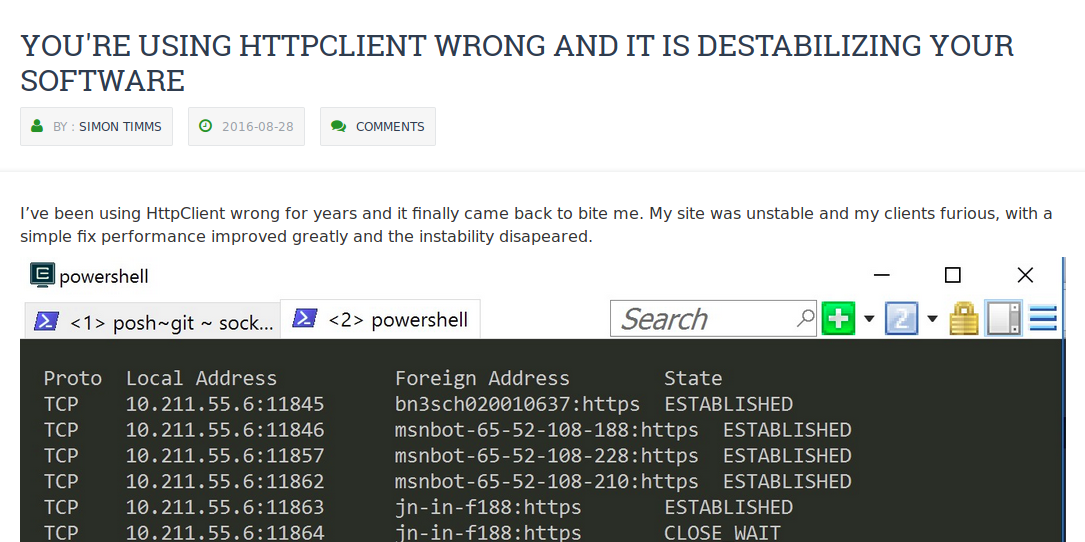
\includegraphics[scale=0.3]{aspnetmonsters}
\end{figure}
\end{frame}

\begin{frame}[fragile]
\frametitle{Проблема socket exhaustion}
\begin{lstlisting}
for(int i = 0; i < 10; i++)
{
  using (var client = new HttpClient())
  {
    await client
      .GetStringAsync("https://api.github.com");
  }
}
\end{lstlisting}
\end{frame}

\begin{frame}
\frametitle{Проблема socket exhaustion}
Проверяем через netstat:
\begin{figure}
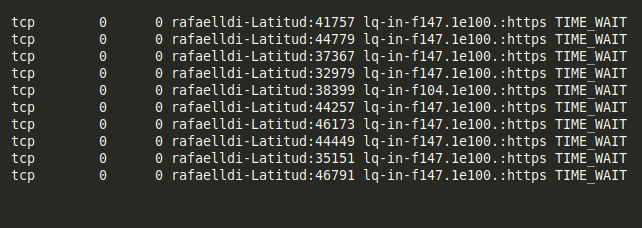
\includegraphics[scale=0.53]{netstat}
\end{figure}
\end{frame}

\begin{frame}
\frametitle{TCP Finite State Machine}
\begin{figure}
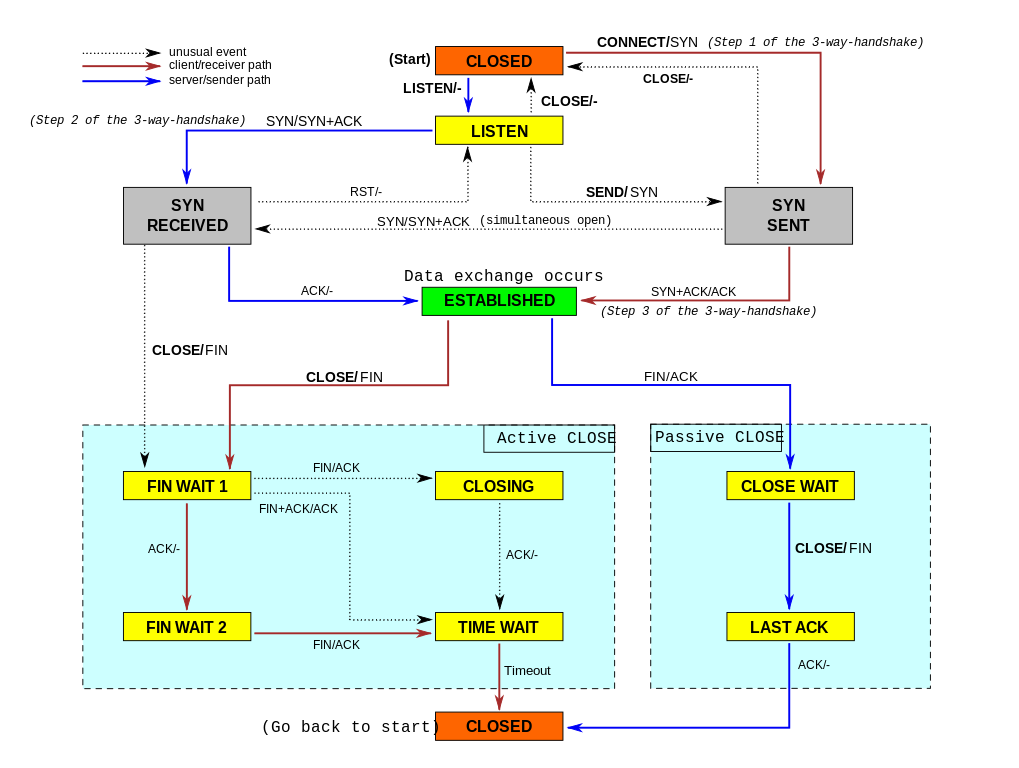
\includegraphics[scale=0.26]{timewait}
\end{figure}
\end{frame}

\begin{frame}
\frametitle{Проблема socket exhaustion}
\begin{itemize}
	\item <1-> 10 сокетов в состоянии \textit{TIME WAIT};
	\item <2-> Приводит к $SocketException$;
	\item <3-> Актуально не только для Windows и .NET Framework.
\end{itemize}
\end{frame}

\begin{frame}
\frametitle{Проблема socket exhaustion}
``HttpClient предназначен для однократного создания экземпляра и повторного использования в течение всего жизненного цикла приложения.''
\newline
\newline
\textit{\href{https://docs.microsoft.com/en-us/dotnet/api/system.net.http.httpclient}{https://docs.microsoft.com/en-us/dotnet/api/system.net.http.httpclient}}
\end{frame}

\begin{frame}[fragile]
\frametitle{Проблема socket exhaustion}
Решение проблемы - переиспользование клиента:
\newline
\begin{lstlisting}
public static HttpClient Client = 
  new HttpClient();
\end{lstlisting}
\end{frame}

\begin{frame}
\frametitle{Проблема кеширования DNS}
\href{https://byterot.blogspot.com/2016/07/singleton-httpclient-dns.html}{https://byterot.blogspot.com/2016/07/singleton-httpclient-dns.html}
\begin{figure}
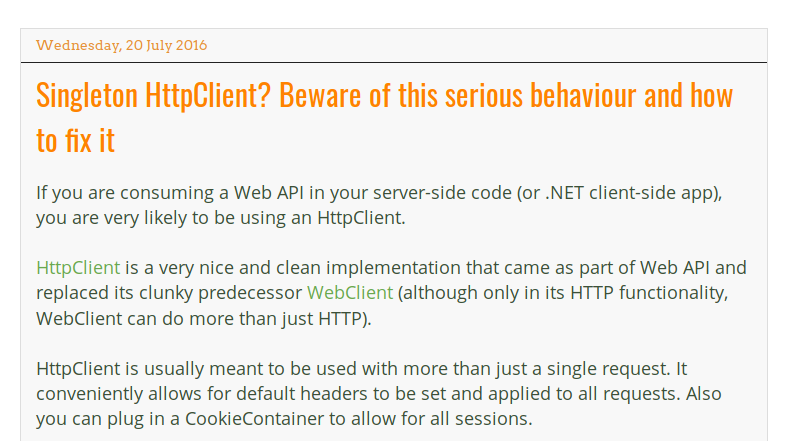
\includegraphics[scale=0.4]{byterot}
\end{figure}
\end{frame}

\begin{frame}
\frametitle{DNS Server}
\begin{figure}
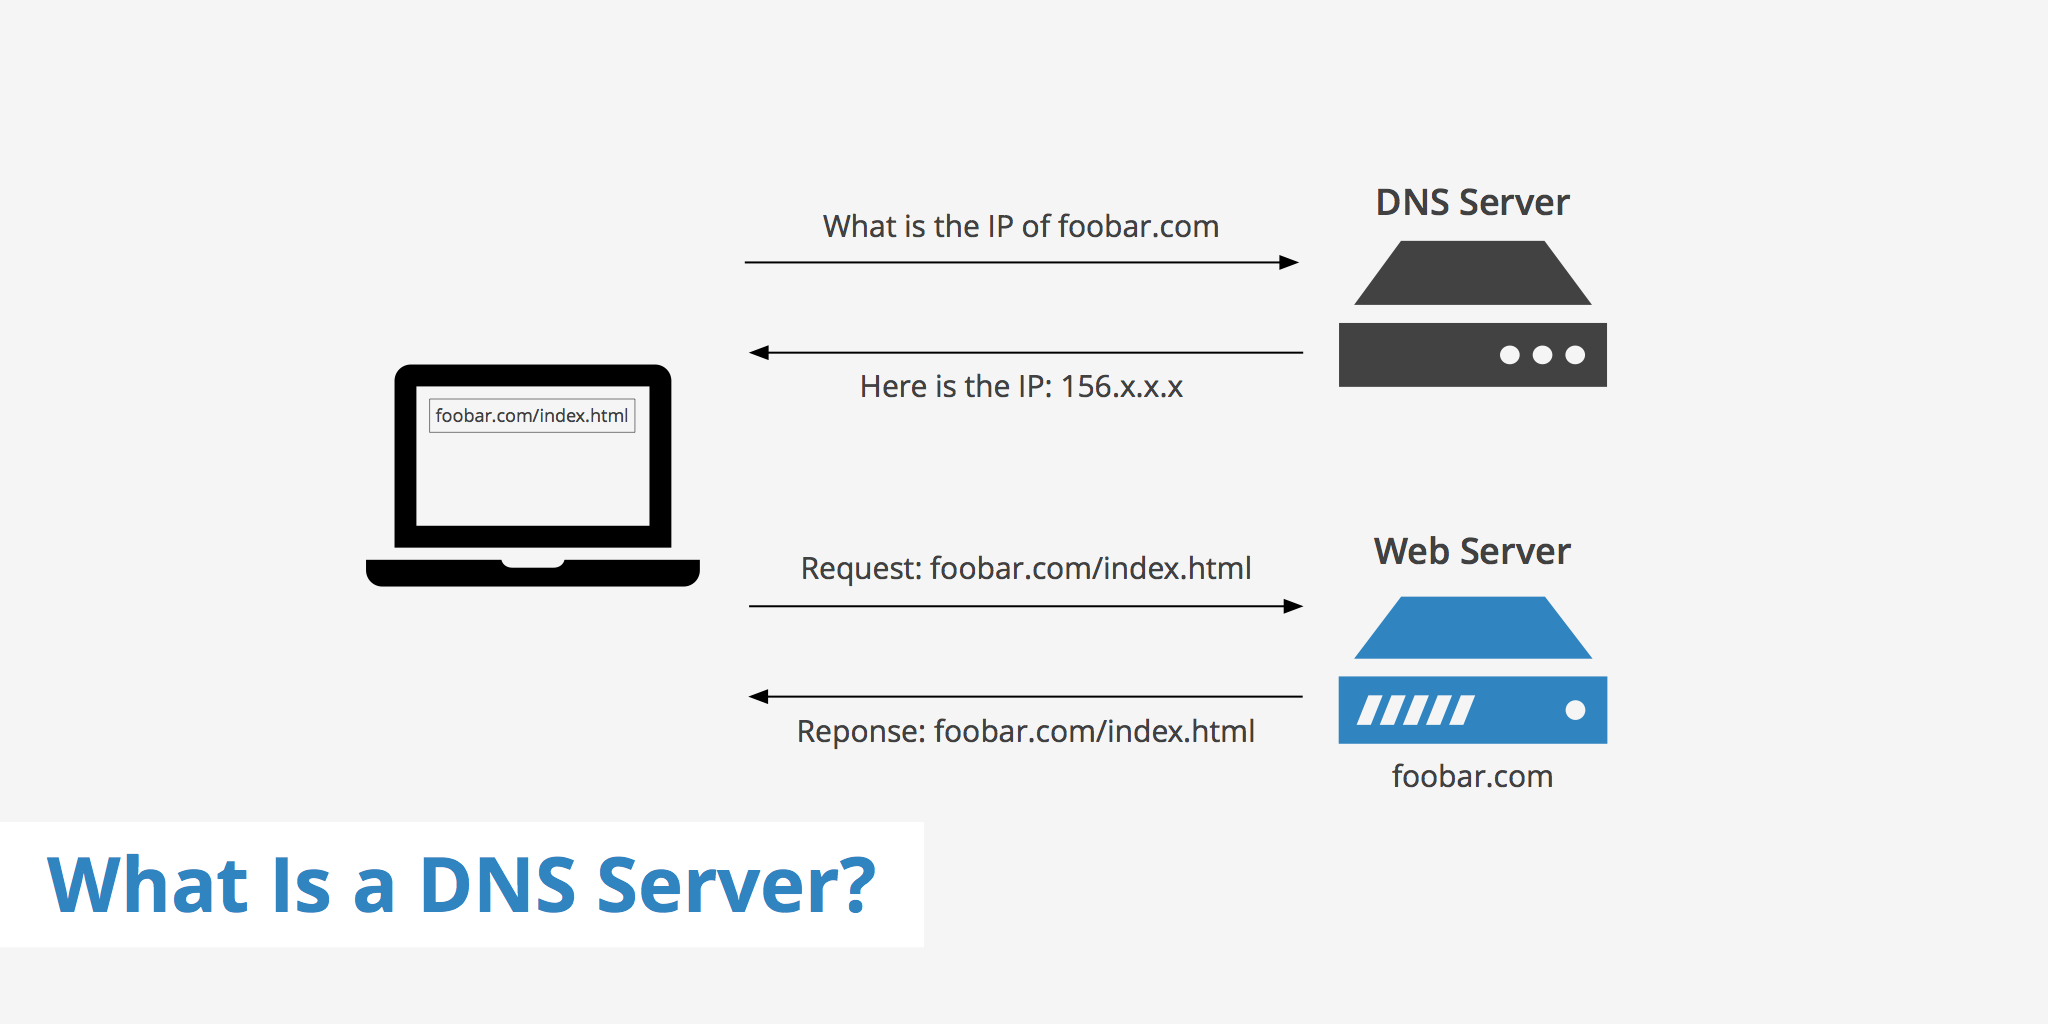
\includegraphics[scale=0.18]{dns}
\end{figure}
\end{frame}

\begin{frame}
\frametitle{Проблема кеширования DNS}
\begin{itemize}
	\item Не учитываются изменения DNS;
	\item Соединение не закрывается длительное время.
\end{itemize}
\end{frame}

\begin{frame}
\frametitle{Проблема кеширования DNS}
Решение для .NET Framework:
\begin{itemize}
	\item <1-> Класс $ServicePointManager$;
	\item <2-> $ServicePointManager.DnsRefreshTimeout$ (2 мин);
	\item <3-> $ServicePoint.ConnectionLeaseTimeout$ (не ограничено);
	\item <4-> $ServicePoint.MaxIdleTime$ (100 сек).
\end{itemize}
\end{frame}

\begin{frame}[fragile]
\frametitle{Проблема кеширования DNS}
Пример:
\begin{lstlisting}
ServicePointManager.DnsRefreshTimeout = 60000;

var sp = ServicePointManager
  .FindServicePoint(
    new Uri("https://api.github.com"));
sp.ConnectionLeaseTimeout = 60000;
sp.MaxIdleTime = 60000;
\end{lstlisting}
\end{frame}

\begin{frame}[fragile]
\frametitle{Quiz}
\begin{lstlisting}
var client = new HttpClient();
var tasks = new List<Task>();
for (var i = 0; i < 20; i++)
{
  tasks.Add(client.GetStringAsync(...));
}
await Task.WhenAll(tasks);
\end{lstlisting}
\end{frame}

\begin{frame}
\frametitle{Quiz}
Сколько одновременных соединений будет установлено?
\newline
\begin{columns}
\column{0.5\textwidth}
\begin{itemize}
\item <1> 1
\item <1> 20
\end{itemize}
\column{0.5\textwidth}
\begin{itemize}
\item <1,2> 2
\item <1> Зависит
\end{itemize}
\end{columns}
\end{frame}

\begin{frame}
\frametitle{Лимит одновременных соединений}
\href{https://habr.com/ru/post/424873/}{https://habr.com/ru/post/424873/}
\begin{figure}
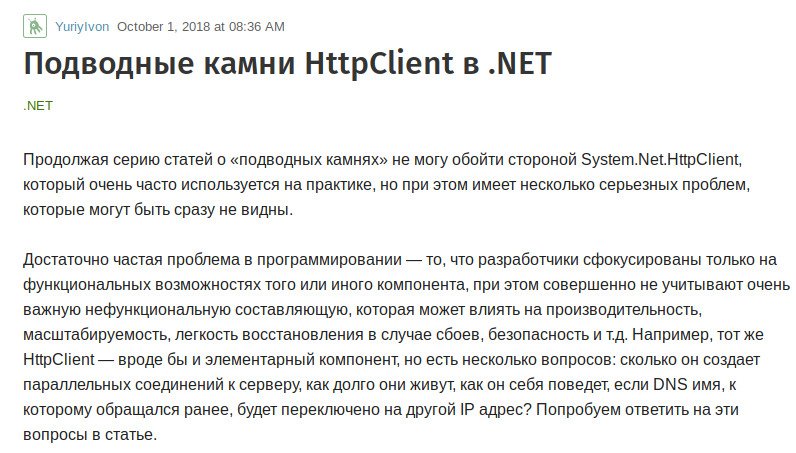
\includegraphics[scale=0.4]{habr}
\end{figure}
\end{frame}

\begin{frame}
\frametitle{Лимит одновременных соединений}
\begin{itemize}
	\item <1-> Лимит по умолчанию равен 2;
	\item <2-> $ServicePointManager.DefaultConnectionLimit$;
	\item <3-> Для $localhost$ по умолчанию равен $int.MaxValue$;
	\item <4-> Только для .NET Framework.
\end{itemize}
\end{frame}

\begin{frame}
\frametitle{Выводы}
\begin{itemize}
	\item <1-> Нельзя на каждый запрос переоткрывать соединение;
	\item <2-> Хочется переиспользовать соединение;
	\item <3-> Нельзя постоянно держать соединение открытым;
	\item <4-> Вручную управлять сложно.
\end{itemize}
\end{frame}

\section{Интерфейс IHttpClientFactory}
\begin{frame}
\frametitle{\href{https://docs.microsoft.com/en-us/dotnet/api/system.net.http.ihttpclientfactory?view=aspnetcore-2.2}{IHttpClientFactory}}
\begin{itemize}
	\item <1-> Позволяет создавать и конфигурировать $HttpClient$;
	\item <2-> Был добавлен в ASP.NET Core 2.1;
	\item <3-> Для консольного приложения необходимо добавить \href{https://www.nuget.org/packages/Microsoft.Extensions.Hosting}{$Microsoft.Extensions.Hosting$} и \href{https://www.nuget.org/packages/Microsoft.Extensions.Http}{$Microsoft.Extensions.Http$}
\end{itemize}
\end{frame}

\begin{frame}[fragile]
\frametitle{IHttpClientFactory}
Регистрация через метод расширения $IServiceCollection$:
\newline
\begin{lstlisting}
services.AddHttpClient();
\end{lstlisting}
\end{frame}

\begin{frame}[fragile]
\frametitle{IHttpClientFactory}
Добавление в конструктор с помощью DI:
\newline
\begin{lstlisting}
public GitHubService(IHttpClientFactory clientFactory)
{
  _clientFactory = clientFactory;
}
\end{lstlisting}
\end{frame}

\begin{frame}[fragile]
\frametitle{IHttpClientFactory}
Создание клиента:
\newline
\begin{lstlisting}
var client = _clientFactory.CreateClient();
var response = await client.SendAsync(request);
\end{lstlisting}
\end{frame}

\begin{frame}[fragile]
\frametitle{Named clients}
Регистрация через метод расширения $IServiceCollection$:
\newline
\begin{lstlisting}
services.AddHttpClient("github", c =>
{
  c.BaseAddress = 
    new Uri("https://api.github.com");
  c.DefaultRequestHeaders
    .Add("Accept", "application/json");
});
\end{lstlisting}
\end{frame}

\begin{frame}[fragile]
\frametitle{Named clients}
Добавление в конструктор с помощью DI:
\newline
\begin{lstlisting}
public SomeService(IHttpClientFactory clientFactory)
{
  _clientFactory = clientFactory;
}
\end{lstlisting}
\end{frame}

\begin{frame}[fragile]
\frametitle{Named clients}
Создание клиента:
\newline
\begin{lstlisting}
var client = _clientFactory.CreateClient("github");
\end{lstlisting}
\end{frame}

\begin{frame}[fragile]
\frametitle{Typed clients}
Класс типизированного клиента:
\begin{lstlisting}
public class GitHubClient
{
  ...
}
\end{lstlisting}
\end{frame}

\begin{frame}[fragile]
\frametitle{Typed clients}
\begin{lstlisting}
private readonly HttpClient _client;
public GitHubClient(HttpClient client)
{
  client.BaseAddress = new Uri("https://api.github.com");
  client.DefaultRequestHeaders.Add("Accept", "application/json");

  _client = client;
}
\end{lstlisting}
\end{frame}

\begin{frame}[fragile]
\frametitle{Typed clients}
\begin{lstlisting}
public async Task<Repo> GetRepo(string repo)
{
  var response = await _client
      .GetAsync($"/repos/octocat/{repo}");
  ...
  return repository;
}
\end{lstlisting}
\end{frame}

\begin{frame}[fragile]
\frametitle{Typed clients}
Регистрация типизированного клиента:
\newline
\begin{lstlisting}
services.AddHttpClient<GitHubClient>();
\end{lstlisting}
\end{frame}

\begin{frame}[fragile]
\frametitle{Typed clients}
Добавление в конструктор через DI:
\newline
\begin{lstlisting}
public GitHubService(GitHubClient gitHubClient)
{
  _gitHubClient = gitHubClient;
}
\end{lstlisting}
\end{frame}

\begin{frame}[fragile]
\frametitle{\href{https://github.com/reactiveui/refit}{Refit}}
Библиотека Refit для REST API (\href{https://github.com/reactiveui/refit}{https://github.com/reactiveui/refit})
\end{frame}

\begin{frame}[fragile]
\frametitle{\href{https://github.com/reactiveui/refit}{Refit}}
\begin{lstlisting}
public interface IGitHubClient
{
  [Get("/repos/octocat/{repo}")]
  Task<Repo> GetRepo(string repo);
}
\end{lstlisting}
\end{frame}

\begin{frame}[fragile]
\frametitle{\href{https://github.com/reactiveui/refit}{Refit}}
Регистрация клиента:
\newline
\begin{lstlisting}
services
  .AddRefitClient<IGitHubClient>()
  .ConfigureHttpClient(c => c.BaseAddress = 
    new Uri("https://api.github.com"));
\end{lstlisting}
\end{frame}

\begin{frame}[fragile]
\frametitle{\href{https://github.com/reactiveui/refit}{Refit}}
Добавление в конструктор через DI:
\newline
\begin{lstlisting}
public GitHubService(IGitHubClient gitHubClient)
{
  _gitHubClient = gitHubClient;
}
\end{lstlisting}
\end{frame}

\begin{frame}[fragile]
\frametitle{Создание HttpClient}
Посмотрим глубже, как происходит создание $HttpClient$
\newline
\begin{figure}

\includegraphics[scale=0.4]{dno}
\end{figure}
\end{frame}

\begin{frame}[fragile]
\frametitle{Создание HttpClient}
\begin{lstlisting}
public class HttpClient : HttpMessageInvoker

public class HttpMessageInvoker : IDisposable

private HttpMessageHandler _handler;
\end{lstlisting}
\end{frame}

\begin{frame}[fragile]
\frametitle{Конструкторы HttpMessageInvoker}
\begin{lstlisting}
public HttpMessageInvoker(HttpMessageHandler handler, bool disposeHandler)

public HttpMessageInvoker(HttpMessageHandler handler) : this(handler, true)
\end{lstlisting}
\end{frame}

\begin{frame}[fragile]
\frametitle{Конструкторы HttpClient}
\begin{lstlisting}
public HttpClient(HttpMessageHandler handler, bool disposeHandler) : base(handler, disposeHandler)

public HttpClient(HttpMessageHandler handler) : this(handler, true)

public HttpClient() : this((HttpMessageHandler) new HttpClientHandler())
\end{lstlisting}
\end{frame}

\begin{frame}
\frametitle{Конструкторы HttpClient}
\begin{itemize}
	\item <1-> 3 конструктора;
	\item <2-> Есть возможность передать $HttpMessageHandler$;
	\item <3-> В стандартном конструкторе $disposeHandler$ равен $true$.
\end{itemize}
\end{frame}

\begin{frame}[fragile]
\frametitle{Dispose HttpClient}
\begin{lstlisting}
protected override void Dispose(bool disposing)
{
  if (disposing && !this._disposed)
  {
    this._disposed = true;
    this._pendingRequestsCts.Cancel();
    this._pendingRequestsCts.Dispose();
  }
  base.Dispose(disposing);
}
\end{lstlisting}
\end{frame}

\begin{frame}[fragile]
\frametitle{Dispose HttpMessageInvoker}
\begin{lstlisting}
public void Dispose()
{
  this.Dispose(true);
  GC.SuppressFinalize((object) this);
}
\end{lstlisting}
\end{frame}

\begin{frame}[fragile]
\frametitle{Dispose HttpMessageInvoker}
\begin{lstlisting}
protected virtual void Dispose(bool disposing)
{
  if (!disposing || this._disposed)
    return;
  this._disposed = true;
  if (!this._disposeHandler)
    return;
  this._handler.Dispose();
}
\end{lstlisting}
\end{frame}

\begin{frame}
\frametitle{Dispose HttpClient}
\begin{itemize}
	\item <1-> Отменяются все повисшие запросы $\Rightarrow$ могут отменяться чужие запросы;
	\item <2-> Не стоит шарить $HttpClient$;
	\item <3-> Флаг $disposed$ выставляется в $true$;
	\item <4-> $Dispose$ вызывается у $HttpMessageHandler$ только в случае $disposeHandler = true$.
\end{itemize}
\end{frame}

\begin{frame}[fragile]
\frametitle{IHttpClientFactory}
\begin{lstlisting}
public static HttpClient CreateClient(
  this IHttpClientFactory factory)
{
  return factory
    .CreateClient(DefaultName);
}
\end{lstlisting}
\end{frame}

\begin{frame}[fragile]
\frametitle{DefaultHttpClientFactory}
\begin{lstlisting}
public HttpClient CreateClient(string name)
{
  HttpClient httpClient = new 
    HttpClient(this.CreateHandler(name), false);
  return httpClient;
}
\end{lstlisting}
\end{frame}

\begin{frame}[fragile]
\frametitle{DefaultHttpClientFactory}
\begin{lstlisting}
public HttpMessageHandler CreateHandler(
  string name)
{
  ActiveHandlerTrackingEntry entry = 
    this._activeHandlers.GetOrAdd(name, this._entryFactory).Value;
  this.StartHandlerEntryTimer(entry);
  return (HttpMessageHandler) entry.Handler;
}
\end{lstlisting}
\end{frame}

\begin{frame}
\frametitle{Создание с помощью HttpClientFactory}
\begin{itemize}
	\item <1-> $Dispose$ не трогает $HttpMessageHandler$;
	\item <2-> $HttpClientFactory$ переиспользует $Handler$;
	\item <3-> $HttpClientFactory$ выставляет таймер для $Handler$;
	\item <4-> Получаем переиспользование соединений.
\end{itemize}
\end{frame}

\begin{frame}
\frametitle{Выводы}
\begin{itemize}
	\item <1-> HttpClientFactory, Named clients, Typed clients, Refit;
	\item <2-> Переиспользуют $HttpMessageHandler$;
	\item <3-> Закрывают $HttpMessageHandler$ спустя время.
\end{itemize}
\end{frame}

\section{Дополнительные улучшения в .NET Core 2.1}
\begin{frame}
\frametitle{\href{https://docs.microsoft.com/en-us/dotnet/api/system.net.http.delegatinghandler?view=netcore-2.2}{DelegatingHandler}}
\begin{itemize}
	\item <1-> $DelegatingHandler$ позволяют создать цепочку обработки исходящих запросов;
	\item <2-> Схоже с middleware в ASP.NET Core;
	\item <3-> Функциональность была, но с $IHttpClientFactory$ стало проще использовать.
\end{itemize}
\end{frame}

\begin{frame}[fragile]
\frametitle{Создание DelegatingHandler}
\begin{lstlisting}
public class SomeHandler : DelegatingHandler
{
  override SendAsync(...)
  {
    ...
    var response = await base.SendAsync(
      request, cancellationToken);
    ...
  }
}     
\end{lstlisting}
\end{frame}

\begin{frame}[fragile]
\frametitle{Пример}
\begin{lstlisting}
override SendAsync(...)
{
  var sw = Stopwatch.StartNew();
  var resp = await base.SendAsync(request, ct);
  sw.Stop();
}     
\end{lstlisting}
\end{frame}

\begin{frame}[fragile]
\frametitle{Пример}
\begin{lstlisting}
override SendAsync(...)
{
  if (!request.Headers.Contains("Key"))
  {
    return new HttpResponseMessage();
  }
  
  return await base.SendAsync(request, ct);
}     
\end{lstlisting}
\end{frame}

\begin{frame}[fragile]
\frametitle{Пример}
\begin{lstlisting}
override SendAsync(...)
{
  return new HttpResponseMessage();
}     
\end{lstlisting}
\end{frame}

\begin{frame}[fragile]
\frametitle{Регистрация DelegatingHandler}
\begin{lstlisting}
services.AddHttpClient("github")
  //first
  .AddHttpMessageHandler<OutsideHandler>()
  //second
  .AddHttpMessageHandler<InsideHandler>()
\end{lstlisting}
\end{frame}

\begin{frame}
\frametitle{\href{https://github.com/App-vNext/Polly}{Polly}}
Библиотека Polly для обработки ошибок (\href{https://github.com/App-vNext/Polly}{https://github.com/App-vNext/Polly})
\begin{figure}

\includegraphics[scale=0.4]{polly}
\end{figure}
\end{frame}

\begin{frame}
\frametitle{\href{https://github.com/App-vNext/Polly}{Polly}}
\begin{itemize}
	\item <1-> Подходит не только для $HttpClient$;
	\item <2-> Содержит различные политики: Retry, Circuit Breaker, Timeout, \ldots
	\item <3-> Необходимо установить \href{https://www.nuget.org/packages/Microsoft.Extensions.Http.Polly/}{$Microsoft.Extensions.Http.Polly$}.
\end{itemize}
\end{frame}

\begin{frame}[fragile]
\frametitle{Добавление политик}
Обработка всех ответов со статус кодами 5xx и 408
\newline
\begin{lstlisting}
services.AddHttpClient("github")
  .AddTransientHttpErrorPolicy(p => p.RetryAsync(3))
  .AddTransientHttpErrorPolicy(
    p => p.CircuitBreakerAsync(5, TimeSpan.FromSeconds(30)));
\end{lstlisting}
\end{frame}

\begin{frame}[fragile]
\frametitle{Настройка внутреннего \href{https://docs.microsoft.com/en-us/dotnet/api/system.net.http.socketshttphandler?view=netcore-2.2}{HttpMessageHandler}}
\begin{lstlisting}
services.AddHttpClient("github")
  .ConfigurePrimaryHttpMessageHandler(() =>
  {
    return new SocketsHttpHandler()
    {
      AutomaticDecompression = DecompressionMethods.GZip
    };
  });
\end{lstlisting}
\end{frame}

\begin{frame}[fragile]
\frametitle{Настройка внутреннего \href{https://docs.microsoft.com/en-us/dotnet/api/system.net.http.socketshttphandler?view=netcore-2.2}{HttpMessageHandler}}
\begin{itemize}
	\item $AllowAutoRedirect$;
	\item $AutomaticDecompression$;
	\item $MaxAutomaticRedirections$;
	\item $MaxResponseHeadersLength$;
	\item \ldots
\end{itemize}
\end{frame}

\begin{frame}[fragile]
\frametitle{Время жизни \href{https://docs.microsoft.com/en-us/dotnet/api/system.net.http.socketshttphandler?view=netcore-2.2}{HttpMessageHandler}}
\begin{lstlisting}
services.AddHttpClient("github")
  .SetHandlerLifetime(TimeSpan.FromMinutes(5));
\end{lstlisting}
\end{frame}

\begin{frame}
\frametitle{Выводы}
\begin{itemize}
	\item Добавились методы для удобной настройки $HttpClient$.
\end{itemize}
\end{frame}


\section{HttpRequestMessage и HttpResponseMessage}
\begin{frame}
\frametitle{\href{https://docs.microsoft.com/en-us/dotnet/api/system.net.http.httprequestmessage?view=netcore-2.2}{HttpRequestMessage}}
Представляет сообщение HTTP-запроса. 
\begin{itemize}
	\item $HttpMethod\,method$;
	\item $Uri\,requestUri$;
	\item $HttpRequestHeaders\,headers$;
	\item $Version\,version$, значение по умолчанию $Version(2, 0)$;
	\item $HttpContent\,content$, который является $IDisposable$;
\end{itemize}
\end{frame}

\begin{frame}[fragile]
\frametitle{Диспозить или нет?}
\begin{enumerate}
	\item <1-> Не диспозить
\begin{lstlisting}
var req = new HttpRequestMessage();
\end{lstlisting}
	\item <2-> Диспозить
\begin{lstlisting}
using(var req = new HttpRequestMessage())
{
  ...                
}
\end{lstlisting}
\end{enumerate}
\end{frame}

\begin{frame}
\frametitle{Диспозить или нет?}
\begin{itemize}
	\item <1-> Зависит от $HttpContent$; 
	\item <2-> Чаще всего это $StringContent$ $\Rightarrow$ можно не диспозить.
\end{itemize}
\end{frame}

\begin{frame}
\frametitle{\href{https://docs.microsoft.com/en-us/dotnet/api/system.net.http.httpresponsemessage?view=netcore-2.2}{HttpResponseMessage}}
Представляет ответное сообщение HTTP.
\begin{itemize}
	\item $HttpStatusCode\,statusCode$ (есть проверка $value > 0$ и $value < 999$);
	\item $HttpResponseHeaders\,headers$;
	\item $string\,reasonPhrase$
	\item $HttpRequestMessage\,requestMessage$
	\item $Version\,version$, значение по умолчанию $Version(1, 1)$;
	\item $HttpContent\,content$, который является $IDisposable$;
\end{itemize}
\end{frame}

\begin{frame}[fragile]
\frametitle{Диспозить или нет?}
\begin{enumerate}
	\item <1-> Не диспозить
\begin{lstlisting}
var resp = await client.GetAsync(...);
\end{lstlisting}
	\item <2-> Диспозить
\begin{lstlisting}
using(var resp = await client.GetAsync(...))
{
  ...                
}
\end{lstlisting}
\end{enumerate}
\end{frame}

\begin{frame}
\frametitle{Диспозить или нет?}
\begin{itemize}
	\item <1-> Для $GetAsync$ и $SendAsync$;
	\item <2-> $HttpCompletionOption$: $ResponseContentRead$, $ResponseHeadersRead$;
	\item <3-> Если $ResponseContentRead$, то данные сохраняются в $MemoryStream$ $\Rightarrow$ можно без диспоза;
	\item <4-> Иначе стоит диспозить. 
\end{itemize}
\end{frame}

\begin{frame}
\frametitle{Всё-таки диспозить или нет?}
\begin{itemize}
	\item <1-> Это внутрення реализация, которая может измениться;
	\item <2-> Лучше всегда диспозить;
	\item <3-> $using\,declarations$.
\end{itemize}
\end{frame}

\begin{frame}[fragile]
\frametitle{Using declarations}
\begin{lstlisting}
using var req = new HttpRequestMessage();

using var resp = await client.GetAsync(...)
\end{lstlisting}
\end{frame}

\begin{frame}[fragile]
\frametitle{Антипаттерн чтения в строку}
\begin{lstlisting}
var response = await client.GetAsync("/repos/octocat/Hello-World");
var str = await response.Content.ReadAsStringAsync();
var repository = JsonConvert.DeserializeObject<Repo>(str);
return repository;
\end{lstlisting}
\end{frame}

\begin{frame}[fragile]
\frametitle{Десериализуем из stream}
\begin{lstlisting}
var srz = new JsonSerializer();
var response = await client.GetAsync("/repos/octocat/Hello-World");
var stream = await response.Content.ReadAsStreamAsync();
using (var sr = new StreamReader(stream))
using (var jsonReader = new JsonTextReader(sr))
{
  return srz.Deserialize<Repo>(jsonReader);
}
\end{lstlisting}
\end{frame}

\begin{frame}[fragile]
\frametitle{Десериализуем из stream в .net core 3.0}
\begin{lstlisting}
var response = await client.GetAsync("/repos/octocat/Hello-World");
var stream = await response.Content.ReadAsStreamAsync();
var repository = await JsonSerializer.DeserializeAsync<Repo>(stream);
return repository;
\end{lstlisting}
\end{frame}

\begin{frame}
\frametitle{Выводы}
\begin{itemize}
	\item <1-> $HttpRequestMessage$ и $HttpResponseMessage$ лучше объявлять, используя $using\,declarations$;
	\item <2-> Лучше не использовать промежуточную строку при десериализации.
\end{itemize}
\end{frame}

\section{Новое в .NET Core 3.0}
\begin{frame}[fragile]
\frametitle{Поддержка HTTP/2}
\begin{lstlisting}
using (var request = 
  new HttpRequestMessage(HttpMethod.Get, "/") 
    { Version = new Version(2, 0) })
\end{lstlisting}
\end{frame}

\begin{frame}[fragile]
\frametitle{Поддержка HTTP/2}
\begin{lstlisting}
var client = new HttpClient()
{
  BaseAddress = new Uri("https://localhost:80"),
  DefaultRequestVersion = new Version(2, 0)
};
\end{lstlisting}
\end{frame}

\begin{frame}[fragile]
\frametitle{Регистрация gRPC Client}
Схожий шаблон с $HttpClient$:
\newline
\begin{lstlisting}
services.AddGrpcClient<GreeterClient>(options =>
{
  options.BaseAddress = new Uri("https://localhost:5001");
});
\end{lstlisting}
\end{frame}

\begin{frame}
\frametitle{Ссылки}
\begin{itemize}
	\item \href{https://aspnetmonsters.com/2016/08/2016-08-27-httpclientwrong/}{You're using HttpClient wrong and it is destabilizing your software};
	\item \href{https://byterot.blogspot.com/2016/07/singleton-httpclient-dns.html}{Singleton HttpClient? Beware of this serious behaviour and how to fix it};
	\item \href{https://nima-ara-blog.azurewebsites.net/beware-of-the-net-httpclient/}{Beware of the .NET HttpClient};
	\item \href{https://habr.com/en/post/424873/}{Подводные камни HttpClient в .NET};
	\item \href{https://docs.microsoft.com/en-us/aspnet/core/fundamentals/http-requests?view=aspnetcore-2.2}{Make HTTP requests using IHttpClientFactory in ASP.NET Core};
	\item \href{https://www.stevejgordon.co.uk}{https://www.stevejgordon.co.uk}.
\end{itemize}
\end{frame}

\begin{frame}
\frametitle{Контакты}
\begin{itemize}
	\item \href{Слайды и примеры https://github.com/rafaelldi/SpbDotNet-HttpClient}{https://github.com/rafaelldi/SpbDotNet-HttpClient};
	\item @rafaelldi;
	\item \href{https://arcadeprogramming.com/}{https://arcadeprogramming.com/}.
\end{itemize}
\end{frame}

\end{document}
